\section{Incremental Search}

For an efficient search in open files, \codeblocks provides the so-called Incremental Search. This search method is initiated for an open file via the menu \menu{Search,Incremental Search} or by the keyboard shortcut Ctrl-I. The focus is then automatically set to the search mask of the corresponding toolbar. As soon as you begin entering the search term, the background of the search mask will be adjusted in accordance with the occurrence of the term. If a hit is found in the active editor, the respective position in the text is marked in colour. By default the current hit will be highlighted in green. This setting can be changed via \menu{Settings, Editor, Incremental Search} (see \pxref{fig:incremental_search_settings}). Pressing the Return key induces the search to proceed to the next occurrence of the search term within the file.

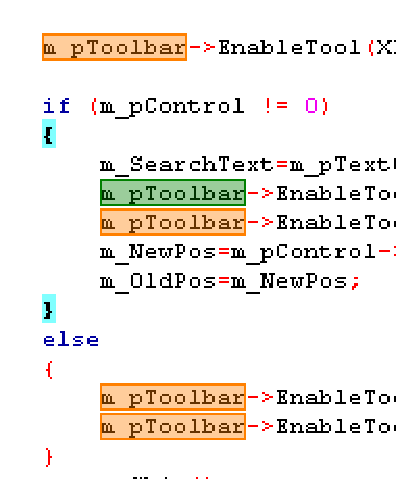
\includegraphics{incremental_search_example}

If the search term cannot be found within the active file, this fact is highlighted by the background of the search mask being displayed in red.

\begin{description}
\item[ESC] Leave the Incremental Search modus.
\item[ALT-DELETE] Clear the input of the incremental search field.
\end{description}

The icons in the Incremental Search toolbar have the following meanings:

\begin{description}
\item[
\includegraphics{incremental_search_clear}] Deleting the text within the search mask of the Incremental Search toolbar.
\item[
\includegraphics{incremental_search_previous},
\includegraphics{incremental_search_next}] Navigating between the occurrences of a search term.
\item[
\includegraphics{incremental_search_highlight}] Clicking this button results in all the occurrences of the search term within the editor being highlighted in colour, instead of only the initial occurrence.
\item[
\includegraphics{incremental_search_selected}] Activating this option restricts the search to the text passage marked within the editor.
\item[
\includegraphics{incremental_search_matchcase}] This option means a case sensitive search is performed.
\end{description}

\hint{The standard settings of this toolbar can be configured in \menu{Settings,Editor,Incremental Search}.}

\screenshot{incremental_search_settings}{Settings for Incremental Search}
